% !TeX root = ./lecture6.tex
% created by Uwe Schadewald
% modified by Mathias Kuntze and Ahmet Uysal
% Add, handout to documentclass arguments for condensed pdf
\documentclass[presentation, 8pt, mathserif, t]{beamer} % , aspectratio=169
\usepackage[english]{babel}
\usepackage{pgf,graphicx}
\usepackage{amsmath, amssymb}
\usepackage[utf8]{inputenc}
\usepackage{lmodern}
\usepackage{palatino}
\usepackage{multimedia}
\usepackage{pgfpages} 
\usepackage{tikz}
\usepackage{datetime}
\pdfoptionpdfminorversion=5

\usepackage{caption}
\usepackage{subcaption}
% if else
\usepackage{ifthen}
% extend table options
\usepackage{tabularx} 
\usepackage{booktabs}
\usepackage{multicol}
\usepackage{multirow}
\usepackage{eso-pic}  % package to set background image
\usepackage[calc]{picture}

% Packages and stuff for ToDo list like itempoints
\usepackage{pifont}
\newcommand{\cmark}{\ding{51}}%
\newcommand{\xmark}{\ding{55}}%
\newcommand{\open}{$\square$}
\newcommand{\done}{\rlap{$\square$}{\raisebox{1pt}{\large\hspace{1.5pt}\cmark}}\hspace{-2.5pt}}
\newcommand{\wontfix}{\rlap{$\square$}{\raisebox{1pt}{\large\hspace{1.5pt}\xmark}}}
\newcommand{\notsure}{\rlap{$\square$}{\raisebox{0.8pt}{\large\hspace{1.5pt}\textbf{?}}}}



% side bar and footer
\setbeamertemplate{headline}{	
	\leavevmode
	\vspace{-4em}	
	\hbox{		
		\begin{beamercolorbox}[wd=0.85\paperwidth,ht=10ex,dp=8ex,center]{}%			
			% navigation with subsections as dots
			\hspace{3.5em}\insertnavigation{0.7\paperwidth}{\hskip0pt plus1fill} % add navigation in footer						
			% navigation with sections, no subsections
			% \insertsectionnavigationhorizontal{0.6\paperwidth}{\hskip0pt plus1fill}{} \\ % add navigation in footer}
			
		\end{beamercolorbox} 				
	}
	\vskip0pt
}


\setbeamertemplate{footline}{	
	\leavevmode
	\vspace{-3em}
	\hbox{
		\begin{beamercolorbox}[wd=.33\paperwidth,ht=2.25ex,dp=1ex,left]{author in head/foot}%
			\hspace{5em}
			\insertshortauthor
		\end{beamercolorbox}
		\begin{beamercolorbox}[wd=.33\paperwidth,ht=2.25ex,dp=1ex,center]{title in head/foot}%
			\insertshorttitle \ - \insertshortsubtitle
		\end{beamercolorbox}	
		\begin{beamercolorbox}[wd=0.30\paperwidth,ht=10ex,dp=8ex,right]{pagenumber in head/foot}			 	
			\insertframenumber % add page numbers
		\end{beamercolorbox}
	}			
	\vskip0pt
}



\setbeamertemplate{frametitle}{
	\ifthenelse{\equal{\insertframesubtitle}{}}{
		\vspace{0.6cm}
		\huge{\insertframetitle}
	}{
		\vspace{0.6cm}
		\small{\insertframetitle}\\
		\vspace{0.3cm}
		\huge{\insertframesubtitle}
    }		
}

	
% enumerate sections
\setbeamertemplate{section in head/foot}{\hfill\insertsectionheadnumber.~\insertsectionhead}
%\setbeamertemplate{section in head/foot shaded}{\color{structure!50}\hfill\insertsectionheadnumber.~\insertsectionhead}
\setbeamertemplate{section in toc}{\inserttocsectionnumber.~\inserttocsection}

%enumerate subsections
\setbeamertemplate{subsection in head/foot}{\hfill\insertsubsectionheadnumber.~\insertsubsectionhead}
\setbeamertemplate{subsection in head/foot shaded}{\color{structure!50}\hfill\insertsubsectionheadnumber.~\insertsubsectionhead}
%\setbeamertemplate{subsection in toc}[subsections numbered]
\setbeamertemplate{subsection in toc}{\vskip0.5em\leftskip=2em\inserttocsubsection\par}

%--------------------------Common------------------------------------------------------
\setbeamercovered{transparent} % make the beamer theme invisible
\usefonttheme{structurebold}
\beamertemplatenavigationsymbolsempty % set navigations helper function to off
\setbeamertemplate{bibliography item}[text]
\setbeamertemplate{note page}[plain]

%\setlist[itemize,1]{label={$\bullet$}} % \item are using bullets
\setbeamertemplate{itemize items}[circle]
	
	

	
% create a new command to show it on two screens
% I'm using dspdfviewer.
\newcommand{\setDualView} {
	\setbeameroption{show notes on second screen=right}
}

%\AtBeginSection[]{\subsection{}}
\newcommand{\addcite}[1]{%
	\AddToShipoutPictureFG*{%
		\AtPageLowerLeft{%
			\put(0.90\paperwidth,5em){											
				\tiny{
					\cite{#1} 
				}			
			}
		}
	}	
}

% insert a frame with references -> use bibtex
\newcommand{\insertReferenceFrame}[3]{%
	\section{#1}
	\begin{frame}[allowframebreaks]
		\frametitle{#1}
		\bibliographystyle{#2}
		\bibliography{#3}
	\end{frame}	
}

\AtBeginSection[]{\subsection{}}
	





\usepackage{../KU-Beamer-Template/style/koc} 
\usepackage{minted}
\usepackage{upquote}
\usepackage{graphicx}
\usepackage{tikz}
\usetikzlibrary{shapes.symbols,positioning, chains}

% pdflatex --shell-escape lecture6.tex & pdflatex --shell-escape lecture6.tex

\title{KOLT Python}
\subtitle{Containers, Aliasing \& Mutability} 
\newdate{date}{04}{11}{2019}
\date{\displaydate{date}}
\author{Gül Sena Altıntaş}

\titlegraphic{
\includegraphics[scale=0.2]{../KU-Beamer-Template/style/images/logo_kolt.pdf}}

\setbeamercovered{invisible} % transparent
\makeatletter
\let\@@magyar@captionfix\relax
\makeatother
\begin{document}
    \maketitle

    \frame{\frametitle{Agenda}\tableofcontents}

    \section{Recap}
    \subsection{Functions}
        \begin{frame}{Functions}
            \Large
            \begin{center}
                \tikzstyle{int}=[draw, fill=blue!20, minimum size=2em]
                \begin{tikzpicture}[node distance=2.5cm,auto]
                    \node [int] (a) {$function$};
                    \node (b) [left of=a,node distance=4cm, coordinate] {a};
                    \node [coordinate] (end) [right of=a, node distance=4cm]{};
                    \path[->] (b) edge node {$*arguments$} (a);
                    \draw[->] (a) edge node {\texttt{return}} (end) ;
                \end{tikzpicture}
            \end{center}
            \pause
            \inputminted[frame=single,framesep=2pt]{python3}{code-examples/function_def.py}
            \pause
            \textbf{\texttt{fib\_100 = fibonacci\_series(100)}}
            \pause
            \textbf{\texttt{what\_is\_going\_on = print(fib\_100)}}
        \end{frame}

        \begin{frame}{return Statement}
            Every function returns one value!\\
            \pause
            What type does each function return?
            % int and string return
            \begin{columns}
                \begin{column}{0.35\textwidth}
                    \pause
                    \inputminted[frame=single, framesep=2pt]{python3}{code-examples/return_int.py}
                \end{column}
                \begin{column}{0.6\textwidth}
                    \pause
                    \inputminted[frame=single, framesep=2pt]{python3}{code-examples/return_string.py}
                \end{column}
            \end{columns}  
            % return none
        \pause
            \inputminted[frame=single, framesep=2pt]{python3}{code-examples/return_none.py}
        % return list
            \pause
            \inputminted[frame=single, framesep=2pt]{python3}{code-examples/return_list.py}
        \end{frame}

    \subsection{Lists}
    \begin{frame}{Sponge Bob seeks for Sandy}
        \pause
        \texttt{cartoon\_characters=['Tweety', 'Mickey', 'Sponge Bob', 'Jerry', 'Minnie']}\\
        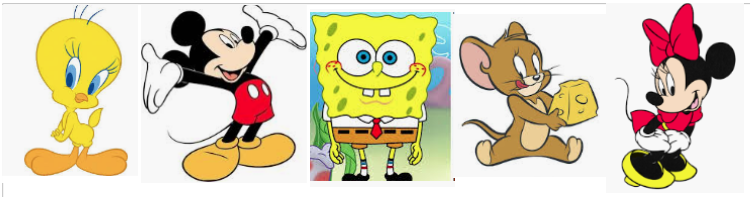
\includegraphics[width=.80\textwidth]{images/list_cartoons/list0.png}   
        \pause
        \texttt{cartoon\_characters.append('Sandy')}\\
        \pause
        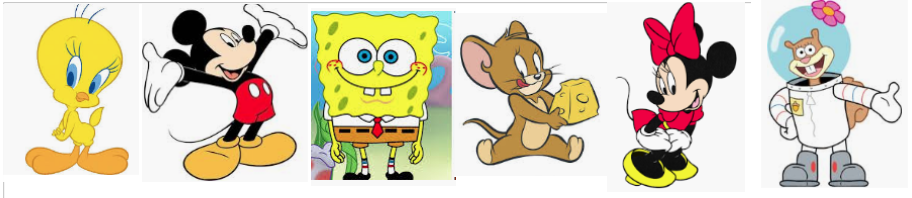
\includegraphics[width=.95\textwidth]{images/list_cartoons/list_after_append.png}       
    \end{frame}

    \begin{frame} {Let's play}
        But, what good is Mickey without being near to Minnie?\\
        \pause
        \texttt{cartoon\_characters.remove('Mickey')}\\
        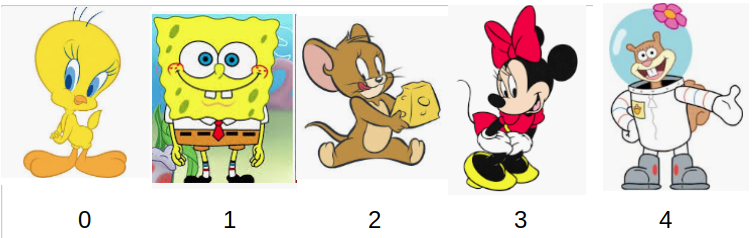
\includegraphics[width=.77\textwidth]{images/list_cartoons/list_after_remove.png}   
        \pause
        \texttt{cartoon\_characters.insert(4, 'Mickey')}\\
        \pause
        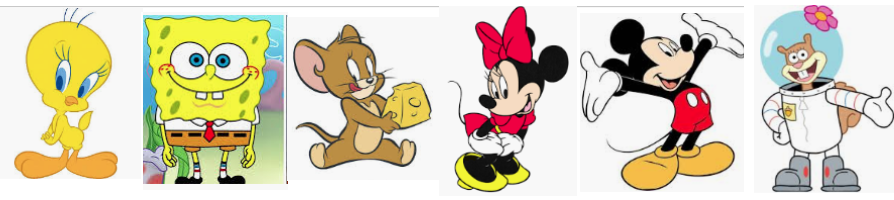
\includegraphics[width=.89\textwidth]{images/list_cartoons/list_after_insert.png}       
    \end{frame}

    \begin{frame}{List Operations}
        Be quick!\\
        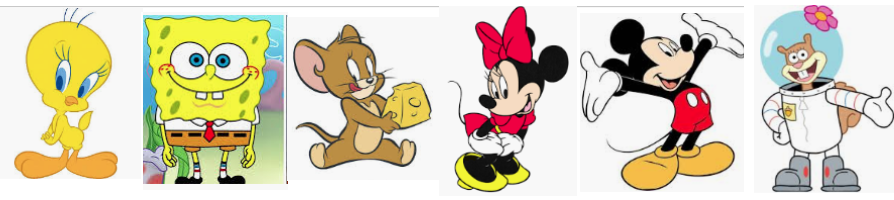
\includegraphics[width=\textwidth]{images/list_cartoons/list_after_insert.png}     
        \texttt{len(cartoon\_characters)}  $\Rightarrow$ \pause 6\\
        \pause \texttt{cartoon\_characters[6]}  $\Rightarrow$ \pause Error\\
        \pause \texttt{'Jerry' in cartoon\_characters}  $\Rightarrow$ \pause False\\
        \pause \texttt{cartoon\_characters.index('Tweety')}  $\Rightarrow$ \pause 0\\
    \end{frame}

    \begin{frame}{Don't let me forget you}
        \pause
        \Large
        Fill out the attendance form: \href{https://tiny.cc/kolt-python}{\underline{\textit{tiny.cc/kolt-python}}}\\
        \pause
            Password: \textbf{Recycle}
        \pause
        \begin{center}
            
\includegraphics[height=0.60\textheight]{images/winnie.jpg}                
        \end{center}
    \end{frame}

    \section{Data Model}
    \begin{frame}{Python Data Model}
        \pause
        \LARGE
        How did we represent data in Python?
        \pause
         \textbf{Variables!}\\
        \pause
        How do they work?
        \pause
         Do they store the data themselves?
        \pause
        \begin{columns}
            \begin{column}{0.5\textwidth}
                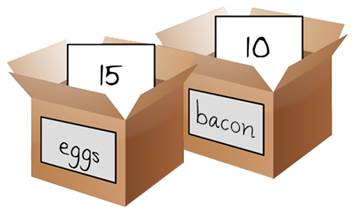
\includegraphics[width=0.9\textwidth]{images/box.jpg}
            \end{column}
            \pause
            \begin{column}{0.5\textwidth}
                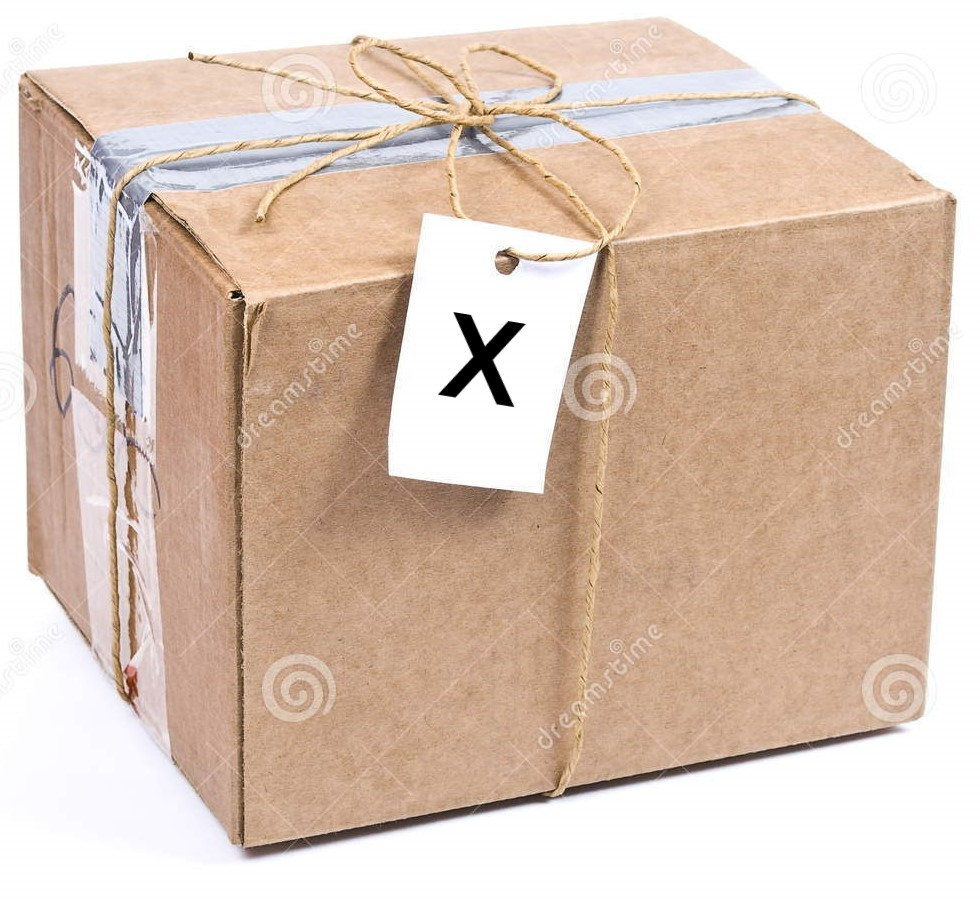
\includegraphics[width=0.6\textwidth]{images/box_tag.jpg}
            \end{column}
        \end{columns}
        
    \end{frame}

    \begin{frame}{Box Analogy}
        \pause
        \inputminted[frame=single,framesep=2pt,firstline=8,lastline=10]{python3}{code-examples/cartoons_box_analogy.py}
        \pause
        \inputminted[frame=single,framesep=2pt,firstline=12, lastline=15]{python3}{code-examples/cartoons_box_analogy.py}
        \pause
        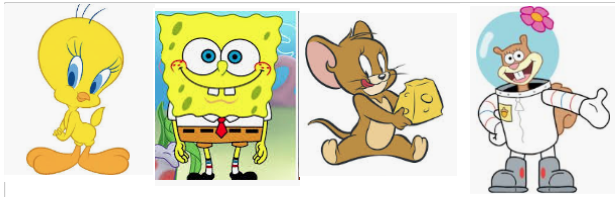
\includegraphics[width=0.66\textwidth]{images/list_cartoons/box_analogy.png}
        \newline
        \pause
        Did we just changed inside of a closed box?\\
        \pause 
         Box analogy \textbf{does not} work!
    \end{frame}

    \begin{frame}{Python Data Model}
       \begin{columns}
            \begin{column}[c]{0.5\textwidth}
                \texttt{cartoon\_characters = ['Tweety', 'Sponge Bob', 'Jerry', 'Minnie', 'Mickey', 'Sandy']}                \\
                \visible<5->{\texttt{mickeys\_leaving = cartoon\_characters}\\}
                \visible<8->{\texttt{mickeys\_leaving.remove('Mickey')}\\}
                \visible<8->{\texttt{mickeys\_leaving.remove('Minnie')}\\}
                \visible<10->{\texttt{print(cartoon\_characters)}}
            \end{column}
            \begin{column}[c]{0.5\textwidth}
                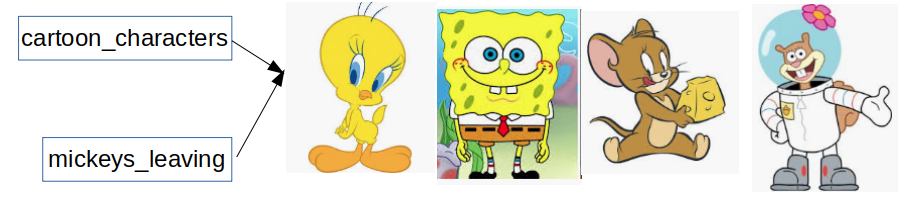
\includegraphics[width=\textwidth]{images/list_cartoons/pointer.png}
                % \begin{tikzpicture}%[node distance=-0.15mm]
                %     \visible<3->{\node[signal, draw, signal from=west, fill=cyan!20] (var1) {cartoon\_characters};}
                %     % \visible<2->{
                %     %     includegraphics[width=0.3\textwidth]{images/list_cartoons/box_analogy.png}
                %     %     % \begin{scope}[start chain, right of= var1, node distance=-.5pt, shift={(1,0)}]
                           
                %     %         % \def\index{2}
                %     %         % \foreach \x in {0,1,2} {
                %     %         %     \ifx\x\index
                %     %         %     \visible<2-8>{\node [draw,on chain] (arr\x) {\x};}
                %     %         %     \else
                %     %         %     \node [draw,on chain] (arr\x) {\x};
                %     %         %     \fi
                %     %         % } 
                %     %     % \end{scope}
                %     % }
                %     \visible<4->{\draw[->] (var1.east) -- (arr0.west);}
                %     \visible<6->{\node[signal, draw, signal from=west, fill=cyan!20, below of=var1] (var2) {mickeys\_leaving};}
                %     \visible<7->{\draw[->] (var2.east) -- (arr0.west);}
                % \end{tikzpicture}
           \end{column}
       \end{columns}
       \bigskip
       \LARGE
       \visible<11->{Variables are more like \textbf{labels} pointing to \textbf{values}!\\}
       \visible<12->{\textbf{Assignment} links \textbf{variables} to \textbf{values}!}
    \end{frame}

   \section{Aliasing \& Cloning}
    \begin{frame}{Aliasing \& Cloning}
        \Large
        \begin{columns}
            \begin{column}[c]{0.6\textwidth}
                \begin{itemize}
                    \item More than one variables can refer to \textbf{same object}!
                    \item What if we want to clone/copy instead of aliasing?
                    \item For lists, \texttt{list.copy()} $\Rightarrow$ returns a \underline{shallow copy} of the list.
                    \item Shallow: only copy the references, not inner values.
                    \item \texttt{>>> import copy}
                \end{itemize}
            \end{column}
            \begin{column}[c]{0.4\textwidth}
                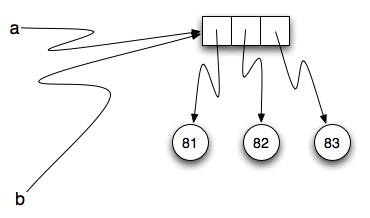
\includegraphics[width=0.9\textwidth]{images/aliasing.png}
            \end{column}
        \end{columns}
    \end{frame}

    \begin{frame}{What if we cloned the cartoon characters}
        \pause
        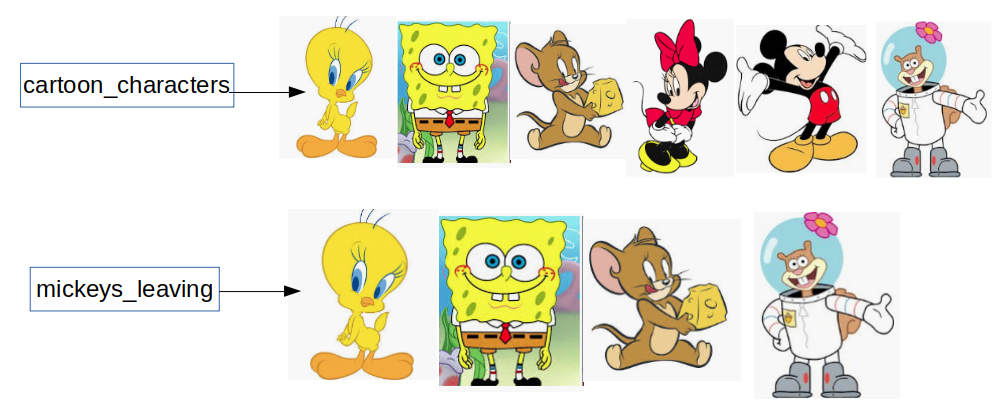
\includegraphics[width=\textwidth]{images/list_cartoons/if_we_cloned.png}
    \end{frame}

    \section{Objects}
    \begin{frame}{Object}
        \LARGE
        \textbf{Everything} is an object in Python.
        \pause
         Even though variables \textbf{do not} have \texttt{types}, each object has a \textbf{fixed} \texttt{type}.\\
        \pause
        $\hookrightarrow$ Values at the right side of our label analogy are objects!
        \bigskip
        \begin{columns}
            \begin{column}[c]{0.5\textwidth}
                \LARGE
                \visible<4->{\texttt{a = 5}\\}
                \visible<8->{\texttt{a = 10}\\}
                \visible<12->{\texttt{a += 3}\\}
                \visible<16->{\texttt{print(a)}}
            \end{column}
            \begin{column}[c]{0.5\textwidth}
                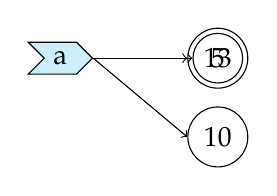
\begin{tikzpicture}%[node distance=-0.15mm]
                    \visible<6->{\node[signal, draw, signal from=west, fill=cyan!20] (var1) {a};}
                    \visible<5-10>{\node[circle, draw, right of=var1, shift={(1,0)}] (val1) {5};}
                    \visible<7-9>{\draw[->] (var1.east) -- (val1.west);}
                    \visible<9-14>{\node[circle, draw, below of=val1] (val2) {10};}
                    \visible<10-13>{\draw[->] (var1.east) -- (val2.west);}
                    \visible<13->{\node[circle, draw, right of=var1, shift={(1,0)}] (val3) {13};}
                    \visible<14->{\draw[->] (var1.east) -- (val3.west);}
                \end{tikzpicture}
           \end{column}
       \end{columns}
    \end{frame}

    \begin{frame}{Object}
        \Large
        Each object has an \texttt{identity},
        \pause
         this value can be obtained by using \texttt{\textbf{id()}} function.\\
        \pause
        \textbf{==} operator compares values, \textbf{\texttt{is}} operator compares identities. 
        \pause
        \inputminted[frame=single,framesep=2pt, firstline=6]{python3}{code-examples/identity.py}
        \pause
        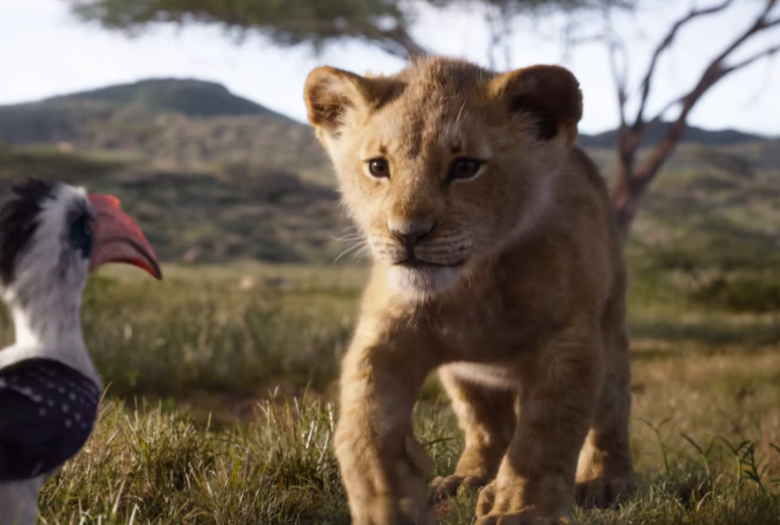
\includegraphics[width=0.25\textwidth]{images/simba_2019.jpg}
        
\includegraphics[width=0.2\textwidth]{images/simba_cartoon.jpg}\\
        Almost always use \textbf{==} to compare values!
    \end{frame}

    \section{Mutability}
    \begin{frame}{Mutability}
        \huge
        \textbf{Immutable:}\\
        \LARGE
        An \texttt{\textbf{object}} with a fixed value.
        \pause
         Immutable objects include \textbf{numbers}, \textbf{strings} and \textbf{tuples}. Such an object cannot be altered.
        \pause
         A new object has to be created if a different value has to be stored.
        \pause
         They play an important role in places where a constant \textbf{hash value} is needed, for example as a \textbf{key} in a \texttt{dictionary}.
        \pause
        \Large
        \begin{columns}
            \begin{column}{0.2\textwidth}
                \inputminted[frame=single,framesep=2pt]{python3}{code-examples/value_update.py}
            \end{column}
            \begin{column}{0.75\textwidth}
                \inputminted[frame=single,framesep=2pt]{python3}{code-examples/change_string.py}
            \end{column}
        \end{columns}
    \end{frame}

    

    \section{Tuples}
    \begin{frame}{Tuples}
        \LARGE
        \begin{itemize}
            \item \textbf{Immutable} sequence(ordered) of elements.
            \pause
            \item Similar to \texttt{list}s, you can use \textbf{indexing}, \textbf{slicing}, and iterate over using \texttt{for} loops.
            \pause
            \item Elements cannot be added/removed/changed once the tuple is created.
            \pause
            \item How to create tuples?
            \pause
             \textbf{\texttt{my\_tuple = (1, [1, 2], \textquotesingle a\textquotesingle )}}
            \pause
            \item \textbf{\texttt{len(my\_tuple)}} $\Rightarrow$
            \pause
             3
            \item \textbf{\texttt{my\_tuple.append(3)}} $\Rightarrow$
            \pause
             \textbf{\texttt{AttributeError:}} \texttt{\textquotesingle tuple\textquotesingle \ object has no attribute \textquotesingle append\textquotesingle}
        \end{itemize}
    \end{frame}

    \begin{frame}{Tuples}
        \LARGE
        \texttt{() / tuple()}: empty tuple, 
        \pause
         \texttt{(3)}:
        \pause
         \texttt{int} 3,
        \pause
         \texttt{(3,)}:
        \pause
         \texttt{tuple} containing 3
        \pause
        \inputminted[frame=single,framesep=2pt]{python3}{code-examples/tuples.py}
    \end{frame}

    \section{Sets}
    \begin{frame}{Sets}
        \LARGE
        \begin{itemize}
            \item \textbf{Unordered} \underline{sequence} of \textbf{unique} elements.
            \pause
            \item \underline{\textbf{Cannot}} use \textbf{indexing/slicing}, \textbf{can} iterate with \texttt{for} loops.
            \pause
            \item \textbf{Mutable}, \texttt{add(element)}, \texttt{remove(element)} methods.
            \pause
            \item Python also has \textbf{immutable} sets: \texttt{frozenset}
            \pause
            \item How to create sets? 
            \pause
             \texttt{my\_set = \{1, 2, 3, 4, 2\}}
            \item How to create empty sets?
            \pause
             \texttt{set()} (\{\ \} is reserved for \texttt{dict})
            \pause
            \item Can compute set operations: \textbf{union}, \textbf{intersection}, \textbf{difference}, \textbf{symmetric difference}.
        \end{itemize}
    \end{frame}
    \begin{frame}{Sets}
        \centering
        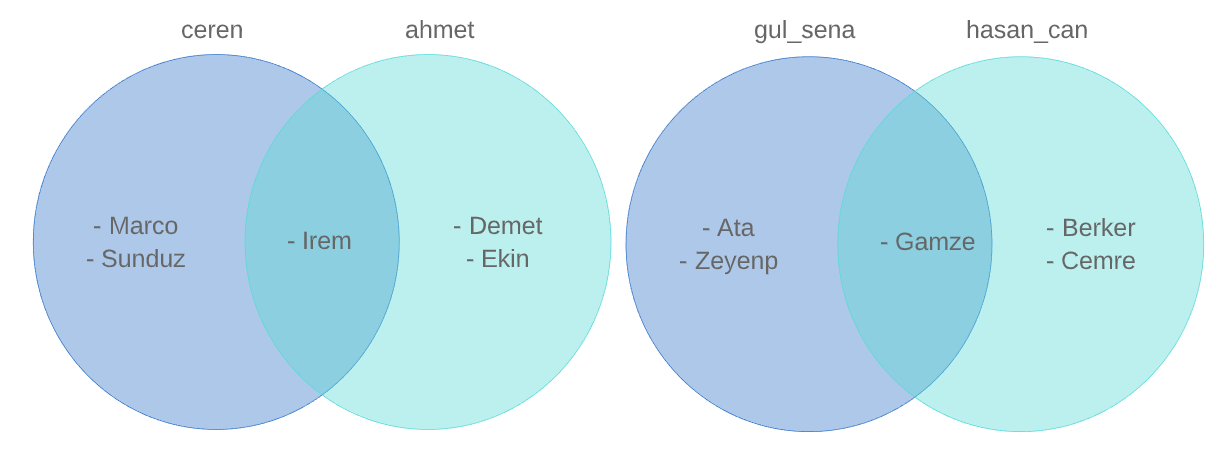
\includegraphics[width=\textwidth]{images/sections_venn.png}
    \end{frame}
    \begin{frame}{Sets}
        \inputminted[frame=single,framesep=2pt]{python3}{code-examples/sets.py}
    \end{frame}
    \section{Dictionaries}
    \begin{frame}{Dictionaries}
        \Large
        \begin{itemize}
            \item Collection of \textbf{key$-$value} \underline{pairs}.
            \pause
            \item \underline{\textbf{Cannot}} use \textbf{indexing/slicing}, \textbf{can} iterate with \texttt{for} loops. 
            \pause
            \item In general, they are not \textbf{ordered}. 
            \pause
            \item However, in Python 3.7 pairs are guaranteed to be in insertion order.
            \pause
            \item In other words, we will get pairs in insertion order if we loop over the \texttt{dict}.
            \pause
            \item How to create dictionaries?
            \pause
             \texttt{\{\ \}/dict()}: empty dictionary
            \pause
            \item \texttt{d = \{\textquotesingle one\textquotesingle : 1, \textquotesingle two\textquotesingle : 2, \textquotesingle three\textquotesingle : 3, \textquotesingle four\textquotesingle : 4\}}
            \pause
            \item How to access values? 
            \pause
             \texttt{print(d[\textquotesingle one\textquotesingle ])} \# $\Rightarrow$ 1
        \end{itemize}
    \end{frame}

    \begin{frame}{Confused Section Leader Gul Sena}
        \inputminted[frame=single,framesep=2pt]{python3}{code-examples/dicts.py}
    \end{frame}

\end{document}